\documentclass{csexp}
\usepackage{hyperref}
\usepackage{todonotes}
\setlength{\marginparwidth}{2cm}

% Define \dd for differential in integrals


\begin{document}


\title{数据结构实验报告}
\expname{线性表实验}


\makecover

\section{实验内容}


\begin{enumerate}
    \item 实现线性表的顺序存储结构和链式存储结构。
    \item 实现线性表的基本操作,包括插入、删除、查找等。
    \item 实现链表的排序操作。
    \item 实现链表的逆序操作。
    \item 实现两个链表的合并操作
\end{enumerate}

\section{程序实现}

\subsection{项目结构}

代码使用\texttt{CMake} 进行构建, 主要包含一下文件:
\begin{verbatim}
    CMakeLists.txt
    main.cpp
    linearList.h
    linearList.cpp
\end{verbatim}

其中, \texttt{main.cpp} 包含了测试代码, \texttt{linearList.h} 包含了线性表的定义, \texttt{linearList.cpp} 包含了线性表的实现。\texttt{CMakeLists.txt} 包含了构建信息。\texttt{CMakeLists.txt}的内容如下:

\begin{lstlisting}[language=CMake]
    cmake_minimum_required(VERSION 3.16)
    project(linear)

    set(CMAKE_CXX_STANDARD 20)

    file(GLOB_RECURSE SOURCE_FILES *.cpp)
    file(GLOB HEADER_FILES *.h)

    add_executable(linear ${SOURCE_FILES} ${HEADER_FILES})
\end{lstlisting}

构建使用如下命令:
\begin{verbatim}
    $ cmake -B build      # generate build files
    $ cmake --build build # build the program
    $ ./build/linear      # run the program
\end{verbatim}

\subsection{顺序表(Sequencial List)}

首先, 定义顺序表的类,包括以下成员变量
\begin{lstlisting}[language=C++]
class sequenceList {
    float *myList;
    int curNumberOfItem;
    int maxCapacity;
}
\end{lstlisting}

分表实现顺序表的\texttt{Constructor}和\texttt{Destructor}函数

\begin{lstlisting}[language=C++]
sequenceList::sequenceList(const int &capacity, const int &length, float initValue[]) {
    myList = new float[capacity]; // allocate memory
    maxCapacity = capacity; // set max capacity
    curNumberOfItem = length; // set current number of items
    memcpy(myList, initValue, length * sizeof(float)); // copy the initial values
}

sequenceList::~sequenceList() {
    delete myList; // free memory
}
\end{lstlisting}

接下来,实现顺序表的基本操作,包括增加、插入、删除操作。

\begin{lstlisting}[language=C++]

bool sequenceList::addItem(const float &newItem) {
    // if the list is full, return false
    if (curNumberOfItem == maxCapacity) {
        return false;
    }
    // add the new item to the end of the list
    myList[++curNumberOfItem] = newItem;
    return true;
}

bool sequenceList::insertItem(const int &idx, const float &newItem) {
    // if the list is full, return false
    if (curNumberOfItem == maxCapacity) {
        return false;
    }
    // move the items after the idx to the right
    for (int i = curNumberOfItem - 1; i > idx; i--) {
        myList[i] = myList[i - 1];
    }
    
    // insert the new item
    curNumberOfItem++;
    myList[idx] = newItem;
    return true;
}


int sequenceList::deleteItem(const float &target) {
    // find the target item
    for (int i = 0; i < curNumberOfItem; i++) {
        if (myList[i] == target) {
            // if found, move the items after the target to the left
            for (int j = i; j < curNumberOfItem - 1; j++) {
                myList[j] = myList[j + 1];
            }

            // decrease the number of items
            curNumberOfItem--;
            return i;
        }
    }
    // if not found, return -1
    return -1;
}
\end{lstlisting}


实现两种查找操作,分别是按值查找和按索引查找。

\begin{lstlisting}[language=C++]
bool sequenceList::locate(const int &idx, float &result) {
    // if the index is out of range, return false
    if (idx < 0 || idx >= curNumberOfItem) {
        return false;
    }
    // return the value at the index
    result = myList[idx];
    return true;
}

int sequenceList::locate(const float &target) {
    // find the target item
    for (int i = 0; i < curNumberOfItem; i++) {
        if (myList[i] == target) {
            // if found, return the index
            return i;
        }
    }
    // if not found, return -1
    return -1;
}
\end{lstlisting}

最后, 实现顺序表的逆序操作, 遍历交换头尾元素。

\begin{lstlisting}[language=C++]
void sequenceList::reverse() {
    int start = 0;
    int end = curNumberOfItem - 1;
    while (start < end) {
        std::swap(myList[start], myList[end]);
        start++;
        end--;
    }
}
\end{lstlisting}

\subsection{有头结点的链表(Linked List with Head Node)}

首先, 定义链表的类,包括以下成员变量

\begin{lstlisting}[language=C++]
class listNode {
    friend class linkList; // For accessing private members

    float data; // Data of the node
    listNode *next; // Pointer to the next node
};

class linkList {
    listNode *firstNode; // Head node
    listNode *curNode; // floating pointer
    listNode *lastNode; // Tail node

    int listSize; // Number of nodes
};
\end{lstlisting}

完成\texttt{listNode}和\texttt{listList}的构造函数和析构函数, 具体实现如下。构造和析构复杂度均为$O(1)$

\begin{lstlisting}[language=C++]


// full args constructor
listNode::listNode(float nodeData, listNode *succ) {
    data = nodeData;
    next = succ;
}

listNode::~listNode() = default;

// constructor with empty list
linkList::linkList(): curNode(nullptr), listSize(0) {
    firstNode = lastNode = new listNode();
}

// constructor with initial values
linkList::linkList(const int &length, float initValue[]): curNode(nullptr), listSize(length) {
    // initial the first node
    lastNode = firstNode = new listNode(0, nullptr); // Initialize the first node as a null header
    listSize = length;

    // Traverse the list and add the initial values
    listNode *current = firstNode;
    for (int i = 0; i < length; i++) {
        current->next = new listNode(initValue[i], nullptr);
        current = current->next;
    }
    lastNode = current; // Update the last node
}

linkList::~linkList() {
    curNode = firstNode;
    // traverse the list and delete the nodes
    while (curNode != lastNode) {
        listNode *nextNode = curNode->next;
        delete curNode;
        curNode = nextNode;
    }
    listSize = 0;
}
\end{lstlisting}

接下来,实现链表的插入操作, 分别是:头插入、尾插入和指定位置插入。 时间复杂度分别为$O(1)$、$O(1)$和$O(n)$

\begin{lstlisting}[language=C++]
bool linkList::headInsertItem(const float &newItem) {
    auto *newNode = new listNode(newItem);
    // re-link the nodes
    newNode->next = firstNode->next;
    firstNode->next = newNode;
    listSize++; // increase the size
    return true;
}

bool linkList::tailInsertItem(const float &newItem) {
    auto *newNode = new listNode(newItem);
    // re-link the nodes
    lastNode->next = newNode;
    lastNode = newNode;
    listSize++; // increase the size
    return true;
}

int linkList::insertItem(const int &idx, const float &newItem) {
    // if the index is out of range, return -1
    if (idx < 0 || idx >= listSize) return -1;
    curNode = firstNode;
    int cnt = 0;
    // traverse the list to the idx
    while (curNode != lastNode) {
        if (cnt == idx) {
            // insert the new node
            auto *newNode = new listNode(newItem);
            newNode->next = curNode->next;
            curNode->next = newNode;
            listSize++;
            return idx;
        }
        curNode = curNode->next;
        cnt++;
    }
    // should not reach here, return -1
    return -1;
}
\end{lstlisting}

实现链表的删除操作,找到对应节点并且重建连接关系。时间复杂度为$O(n)$

\begin{lstlisting}[language=C++]

int linkList::deleteItem(const float &target) {
    curNode = firstNode;
    int cnt = 0;
    // traverse the list to find the target
    while (curNode != lastNode) {
        if (curNode->next->data == target) {
            //re-link the nodes
            const listNode *tmp = curNode->next;
            curNode->next = curNode->next->next;
            delete tmp; // free the memory
            listSize--; // decrease the size
            return cnt; // return the index
        }
        curNode = curNode->next;
        cnt++;
    }
    // if not found, return -1
    return -1;
}
\end{lstlisting}

实现链表的查找操作,分别是按值查找和按索引查找。时间复杂度分别为$O(n)$和$O(n)$

\begin{lstlisting}[language=C++]

// locate by index
bool linkList::locate(const int &idx, float &val) {
    curNode = firstNode;
    int cnt = 0;
    // traverse the list to the idx
    while (curNode != lastNode) {
        if (cnt == idx) {
            val = curNode->next->data; // put the value to the val
            return true; // return true if found
        }
        curNode = curNode->next; // move to the next node
        cnt++;
    }
    return false; // if not found, return false
}

// locate by value
int linkList::locate(const float &target) {
    curNode = firstNode;
    int cnt = 0;
    // traverse the list to find the target
    while (curNode != lastNode) {
        if (curNode->next->data == target) {
            // if found, return the index
            return cnt;
        }
        curNode = curNode->next;
        cnt++;
    }
    // if not found, return -1
    return -1;
}
\end{lstlisting}

实现链表的排序操作, 这里使用归并排序算法,使用快慢指针找到中间节点,然后递归排序,合并序列。
排序完成之后,更新尾节点。排序时间复杂度为$O(n\log n)$

\begin{lstlisting}[language=C++]
void linkList::ascendingOrder() {
    firstNode->next = mergeSort(firstNode->next);<
    while (lastNode->next != nullptr) {
        lastNode = lastNode->next;
    }
}

listNode *linkList::mergeSort(listNode *head) {
    if (!head || !head->next) {
        return head;
    }

    // fast-slow pointer to find the middle node
    listNode *slow = head;
    listNode *fast = head->next;
    while (fast && fast->next) {
        slow = slow->next;
        fast = fast->next->next;
    }

    listNode *mid = slow->next;
    slow->next = nullptr;

    // recursively sort the left and right part
    listNode *left = mergeSort(head);
    listNode *right = mergeSort(mid);

    // merge the left and right part
    return orderedMerge(left, right);
}

// 合并两个已排序链表的函数
listNode *linkList::orderedMerge(listNode *left, listNode *right) {
    listNode dummy;
    listNode *tail = &dummy;

    while (left && right) {
        if (left->data < right->data) {
            tail->next = left;
            left = left->next;
        } else {
            tail->next = right;
            right = right->next;
        }
        tail = tail->next;
    }

    tail->next = left ? left : right;
    return dummy.next;
}
\end{lstlisting}

实现链表的逆序操作, 遍历交换头尾元素,重建连接关系。时间复杂度为$O(n)$

\begin{lstlisting}[language=C++]
void linkList::reverse() {
    listNode *prev = nullptr;
    listNode *current = firstNode->next; // Skip the null header
    listNode *next = nullptr;
    lastNode = current; // The current first node will become the last node
    // traverse the list 
    while (current != nullptr) {
        // re-link the nodes with reverse order
        next = current->next;
        current->next = prev;
        prev = current;
        current = next;
    }
    firstNode->next = prev; // Update the first node
}
\end{lstlisting}

实现两个链表的合并操作, 首先排序, 然后合并。时间复杂度为$O(n\log n)$

\begin{lstlisting}[language=C++]
void merge(linkList &A, linkList &B) {
    // sort the two lists
    A.ascendingOrder();
    B.ascendingOrder();
    // merge the two lists
    A.firstNode->next = linkList::orderedMerge(A.firstNode->next, B.firstNode->next);
    // update the last node for A
    while (A.lastNode->next != nullptr) {
        A.lastNode = A.lastNode->next;
    }
    // disconnect the list B
    B.firstNode->next = nullptr;
    // update the size
    A.listSize += B.listSize;
    B.listSize = 0;
}
\end{lstlisting}


\section{实验结果}
\subsection{顺序表测试}
使用如下代码测试顺序表的基本操作, 使用\texttt{assert}函数进行断言,使更容易发现错误。所有测试通过。

\begin{lstlisting}[language=C++]
// Link List Test Cases
{
    float i[3] = {1.3, 4.5, 0.4};
    float val;
    linkList ll(3, i);
    ll.print(); // 3:1.3,4.5,0.4
    ll.tailInsertItem(5.5);
    ll.print(); // 4:1.3,4.5,0.4,5.5
    ll.headInsertItem(7);
    ll.print(); // 5:7,1.3,4.5,0.4,5.5
    assert(ll.deleteItem(1.3f) == 1); //返回1
    ll.print(); // 4: 7,4.5,0.4,5.5
    assert(!ll.locate(9, val)); //返回false
    assert(ll.locate(4.5f) == 1); //返回1
    ll.print(); // 4:7, 4.5,0.4,5.5
    ll.reverse(); //
    ll.print(); // 4: 5.5,0.4,4.5,7
    ll.insertItem(1, 10.2f);
    ll.print(); // 5: 5.5,10.2,0.4,4.5,7
}
\end{lstlisting}

该部分代码的输出如图~\ref{fig:seq-test}所示。

\begin{figure}[htbp]
    \centering
    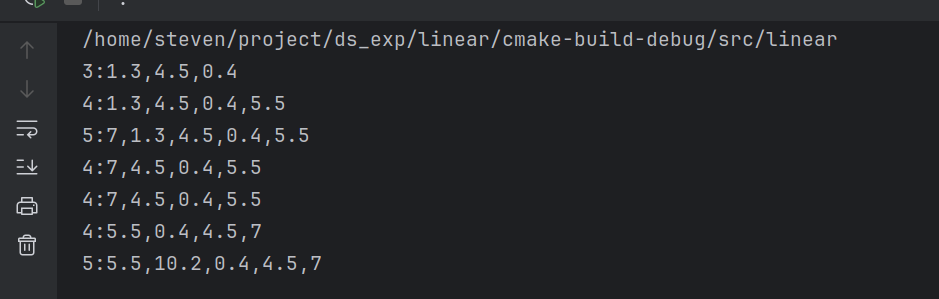
\includegraphics[width=0.8\textwidth]{exp1-1.png}
    \caption{顺序表测试结果}
    \label{fig:seq-test}
\end{figure}

\subsection{链表测试}

使用如下代码测试链表的基本操作, 同样使用\texttt{assert}函数进行断言。

\begin{lstlisting}[language=C++]
// Sequence List Test Cases
{
    float i[3] = {1.3, 4.5, 0.4};
    float val;
    sequenceList sl(50, 3, i); // 顺序表容量,初始化数组长度,初始化数组值

    sl.print(); // 3:1.3,4.5,0.4
    sl.locate(0, val);
    assert(sl.locate(0, val) && val == 1.3f);
    assert(sl.locate(1, val) && val == 4.5f);
    assert(sl.locate(2, val) && val == 0.4f);

    sl.insertItem(3, 5.5);
    sl.print(); // 4:1.3,4.5,0.4,5.5
    assert(sl.locate(3, val) && val == 5.5f);

    sl.deleteItem(1.3); // 返回0
    sl.print(); // 3: 4.5,0.4,5.5
    assert(sl.locate(0, val) && val == 4.5f);
    assert(sl.locate(1, val) && val == 0.4f);
    assert(sl.locate(2, val) && val == 5.5f);

    assert(!sl.locate(9, val)); // 返回false
    assert(sl.locate(4.5) == 0); // 返回0

    sl.print(); // 3: 4.5,0.4,5.5

    sl.reverse();
    sl.print(); // 3: 5.5,0.4,4.5
    assert(sl.locate(0, val) && val == 5.5f);
    assert(sl.locate(1, val) && val == 0.4f);
    assert(sl.locate(2, val) && val == 4.5f);
}
\end{lstlisting}

该部分代码的输出如图~\ref{fig:link-test}所示。

\begin{figure}[htbp]
    \centering
    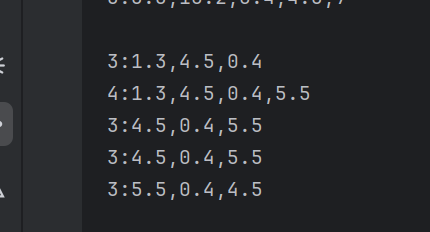
\includegraphics[width=0.8\textwidth]{exp1-2.png}
    \caption{链表测试结果}
    \label{fig:link-test}
\end{figure}

最后,进行排序和合并操作的测试, 代码如下:

\begin{lstlisting}[language=C++]
// Sort and Merge Test Cases
{
    float a[3] = {1.3, 4.5, 0.4};
    float b[4] = {1.5, 8.5, 0.1, 6.2};
    linkList alist(3, a);
    linkList blist(4, b);

    alist.print(); // 3:1.3,4.5,0.4
    blist.print(); // 4:1.5,8.5,0.1,6.2

    alist.ascendingOrder();
    blist.ascendingOrder();

    alist.print(); // 3:0.4,1.3,4.5
    blist.print(); // 4:0.1,1.5,6.2,8.5

    merge(alist, blist);

    alist.print(); // 7:0.1,0.4,1.3,1.5,4.5,6.2,8.5
}
\end{lstlisting}

该部分代码的输出如图~\ref{fig:sort-merge}所示。

\begin{figure}[htbp]
    \centering
    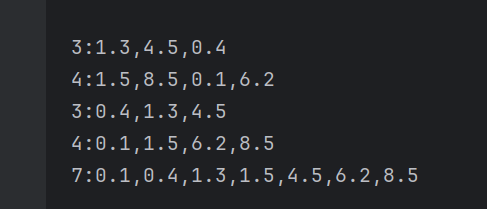
\includegraphics[width=0.8\textwidth]{exp1-3.png}
    \caption{排序和合并测试结果}
    \label{fig:sort-merge}
\end{figure}

\section{实验中遇到的问题及解决方法}

\begin{enumerate}
    \item \textbf{内存泄漏问题}: 在链表的析构函数中, 需要释放所有节点的内存, 但是如果不小心忘记释放, 就会导臃内存泄漏。解决方法是在析构函数中使用循环遍历所有节点, 释放内存。
    \item \textbf{快慢指针}: 因为无法随机访问,需要使用快慢指针找到中间节点。
    \item \textbf{尾节点的更新}:排序与合并之后需要更新尾节点,不然无法正确维护数据结构和输出。
\end{enumerate}

\end{document}